%---------------------------------------------------------------------
% Course 	: Introduction To web sciences
% Professor : Dr.Nelson
% Name   	: Msnoj Chandra Kompalli
% Assignment: 5
%---------------------------------------------------------------------
\documentclass[12pt]{article}
%--------------------------------------------------------------------
% packages required
%--------------------------------------------------------------------
\usepackage{graphicx}
\usepackage{listings}
\usepackage{hyperref}
\usepackage{caption}
\usepackage{color}
\usepackage{pdfpages}
\graphicspath{ {images/} }
%--------------------------------------------------------------------
% Start Margins
%--------------------------------------------------------------------
\addtolength{\oddsidemargin}{-.875in}
\addtolength{\evensidemargin}{-.875in}
\addtolength{\textwidth}{1.75in}
\addtolength{\topmargin}{-.885in}
\addtolength{\textheight}{1.95in}
%-------------------------------------------------------------------
% End Margins
%--------------------------------------------------------------------
\definecolor{codegreen}{rgb}{0,0.6,0}
\definecolor{codegray}{rgb}{0.5,0.5,0.5}
\definecolor{codepurple}{rgb}{0.58,0,0.82}
\definecolor{backcolour}{rgb}{0.95,0.95,0.92}
 
\lstdefinestyle{mystyle}{
    backgroundcolor=\color{backcolour},   
    commentstyle=\color{codegreen},
    keywordstyle=\color{magenta},
    numberstyle=\tiny\color{codegray},
    stringstyle=\color{codepurple},
    basicstyle=\footnotesize,
    breakatwhitespace=false,         
    breaklines=true,                 
    captionpos=b,                    
    keepspaces=true,                 
    numbers=left,                    
    numbersep=5pt,                  
    showspaces=false,                
    showstringspaces=false,
    showtabs=false,                  
    tabsize=2
}
 
\lstset{style=mystyle}

\begin{document}

\begin{titlepage}
\title{INTRODUCTION TO WEB SCIENCES:\\*Assignment 5}
\author{Manoj Chandra Kompalli}
\date{3 March 2016}
\maketitle
\end{titlepage}

\tableofcontents
\newpage

\section{Question 1:  }
  We know the result of the Karate Club (Zachary, 1977) split.
Prove or disprove that the result of split could have been predicted
by the weighted graph of social interactions.  How well does the
mathematical model represent reality?

Generously document your answer with all supporting equations, code,
graphs, arguments, etc.

\subsection{Understanding}
It was a real tough time to understand what was expected from me to show. I had understood that I should show the difference between actual split and predicted split and prove they are almost same. There are a few algorithms that can predict the split of Karate problem. Here a Karate group is split into two due to some issues. Some people join one group and some join the other. Rest of them do not join any group. We want to predict using the algorithm, who joins which group.\par In a graph, vertices represent the people and edges represent the contact. People having strong contact with their leader ideally choose that group. Mathematically, this can be proved by a few algorithms. Through a bit of research, I found out that Girvan-Newman Algorithm for edge betweenness is one of the most accurate around. Betweenness centrality is an indicator of a node's centrality in a network. It is equal to the number of shortest paths from all vertices to all others that pass through that node. A node with high betweenness centrality has a large influence on the transfer of items through the network, under the assumption that item transfer follows the shortest paths. According to this algorithm, we have to find the edge with maximum betweenness and delete it. We have to iterate the process until we get two groups. 

\subsection{Implementation}
\begin{itemize}  
\item I had to download the karate graphML .
\item Install the igraph library for python
\item Install pycairo for igraph. 
\item Load the graph
\item Find edge betweeness of graph 
\item Find the edge with maximum edge betweenness
\item Delete the edge
\item Repeat the process until you make two clusters
 
\end{itemize}
 \newpage

\subsection{Code Listing}
\subsubsection{karateGroup.py}
\lstinputlisting[breaklines=True,language=Python]{../qn1/karateGroup.py}
\newpage

\subsection{Input}
\subsubsection{karate.GraphML}
\lstinputlisting[breaklines=True]{../qn1/samplegraphML.GraphML}

\newpage


\subsection{Summary and Output}
Figure~\ref{fig:initial-graph} is the initial graph generated from the karate.GraphML. The initial graph consists of all the vertices generated from karate graphML. The actual graph in Figure~\ref{fig:Actual Seperation of Groups} shows actual  separation of 34 members into two groups based on faction data. Blue belong to Mr. Hi and the pink belong to John. By comparing it with Figure~\ref{fig:Predicted Seperation using Edge betweenness}. By careful observation, we can see that only the actor 3 who was predicted to be in Mr. John ’s group is actually in Mr. Hi's group. This proves that our prediction using the algorithm is near perfect. We can use this model to predict the number of groups in a real world social network. 
\subsubsection{Initial Graph}
\begin{figure}[ht]
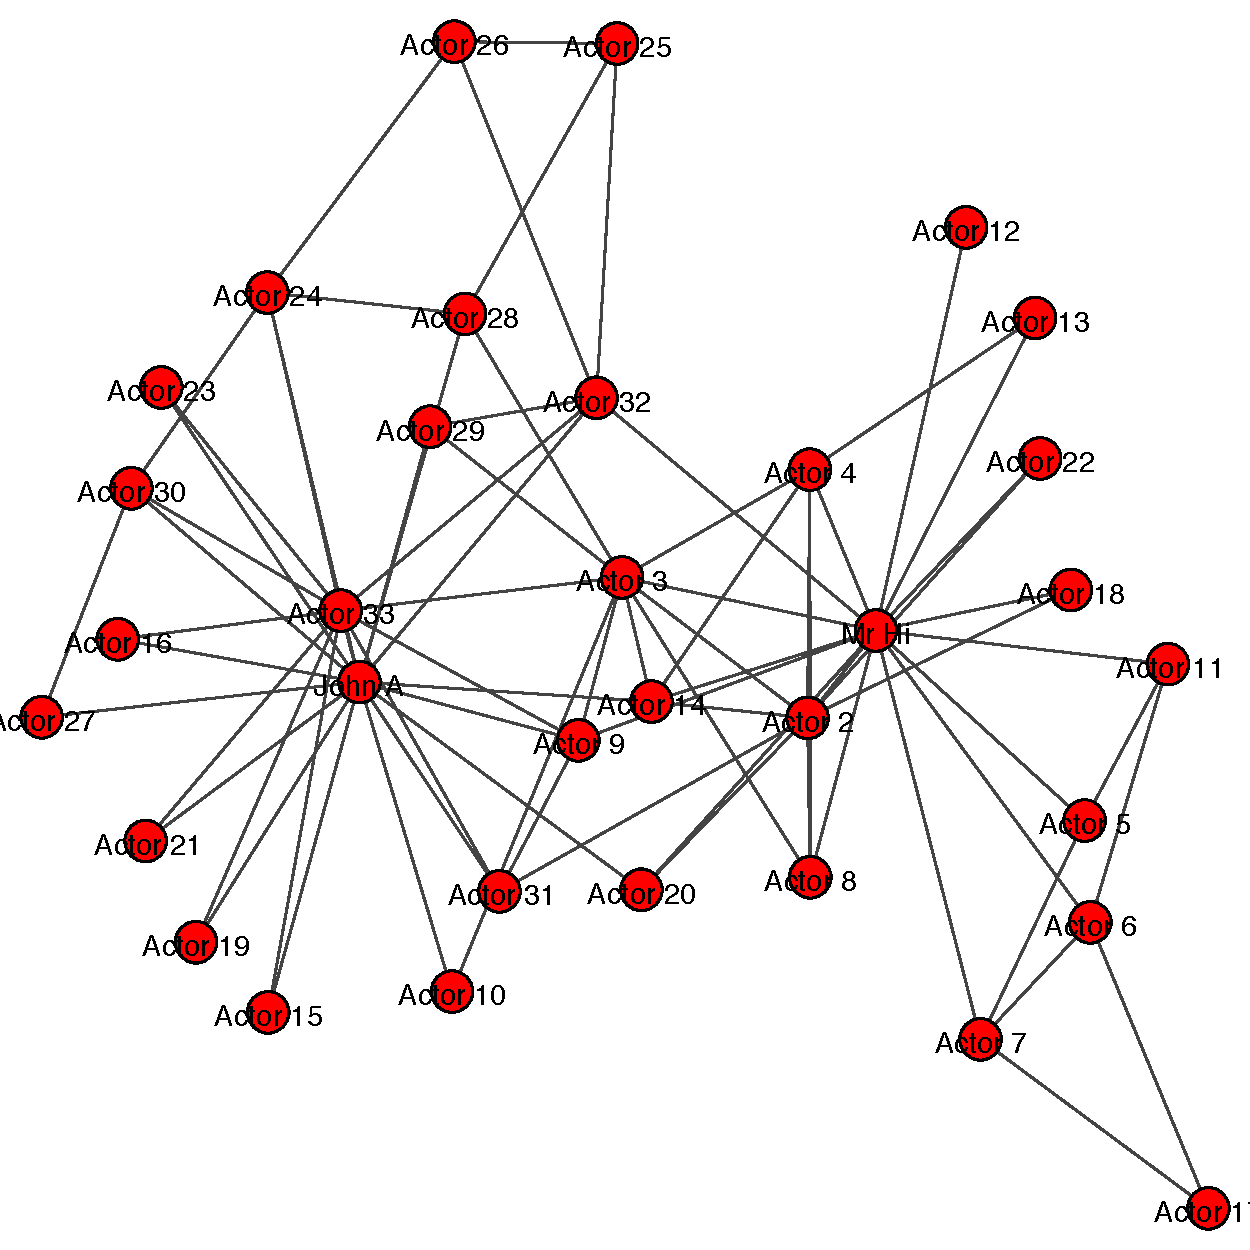
\includegraphics[scale=0.7]{../qn2/graph3.pdf}
\centering
\caption{initial-graph}
\label{fig:initial-graph}
\end{figure}
\newpage
\subsection{Processed graphs}
\subsubsection{Graph showing actual division based on Faction}

\begin{figure}[ht]
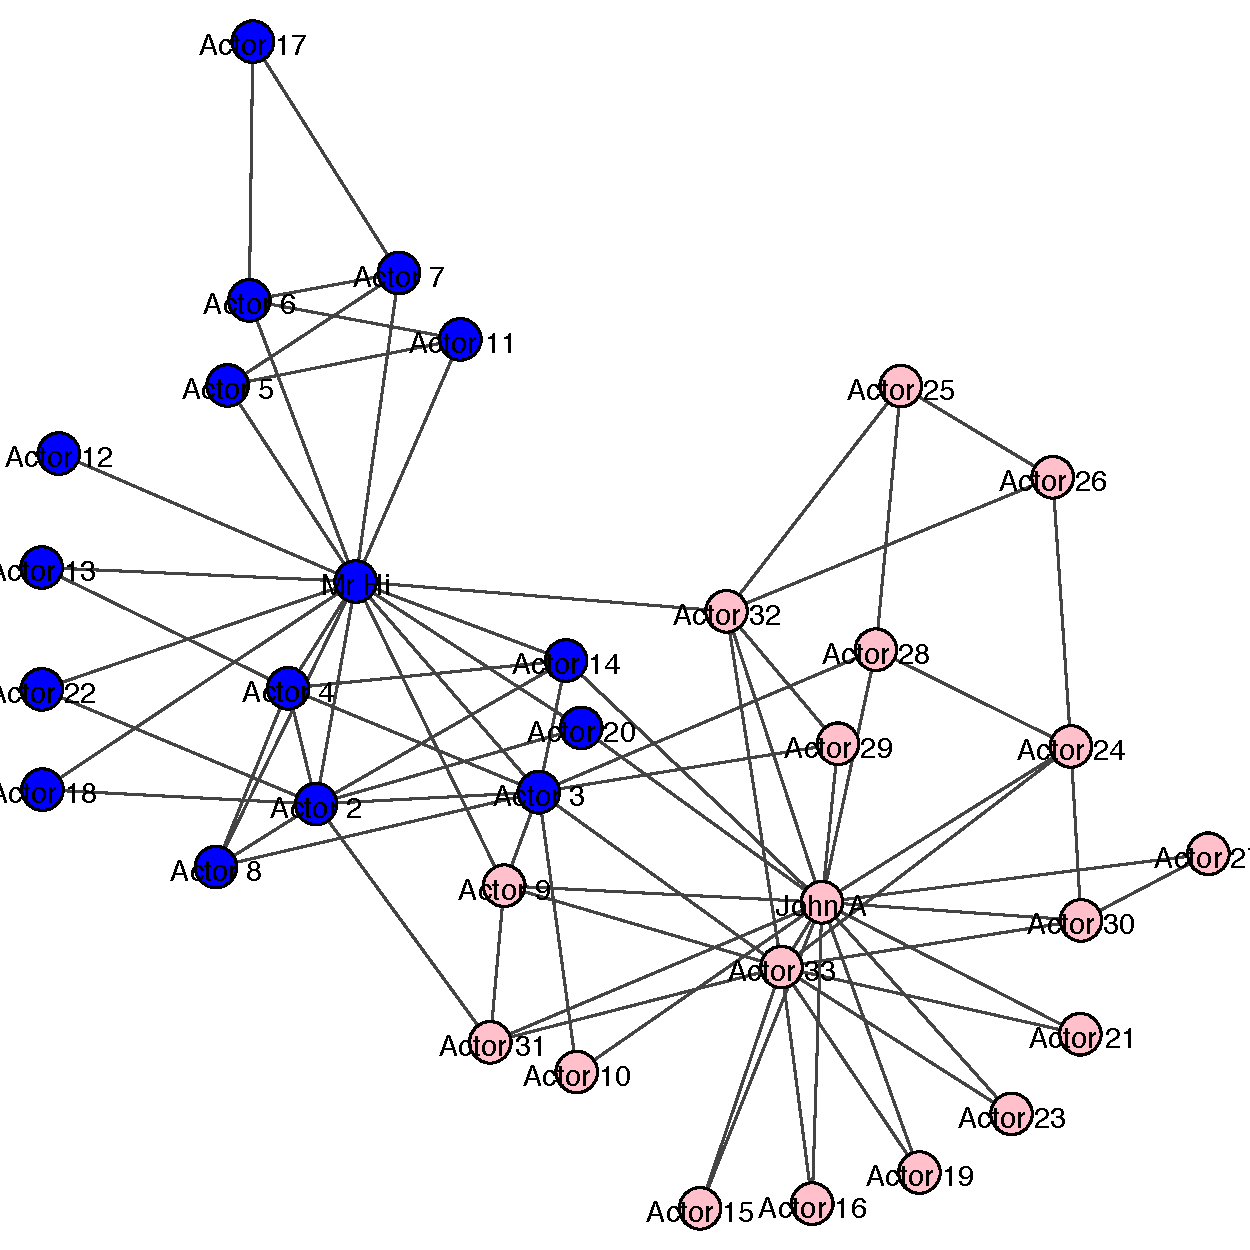
\includegraphics[scale=0.7]{../qn1/graphkk.pdf}
\centering
\caption{Actual Seperation of Groups}
\label{fig:Actual Seperation of Groups}
\end{figure}
\newpage
\subsubsection{Graph showing actual division based on Faction}
\begin{figure}[ht]
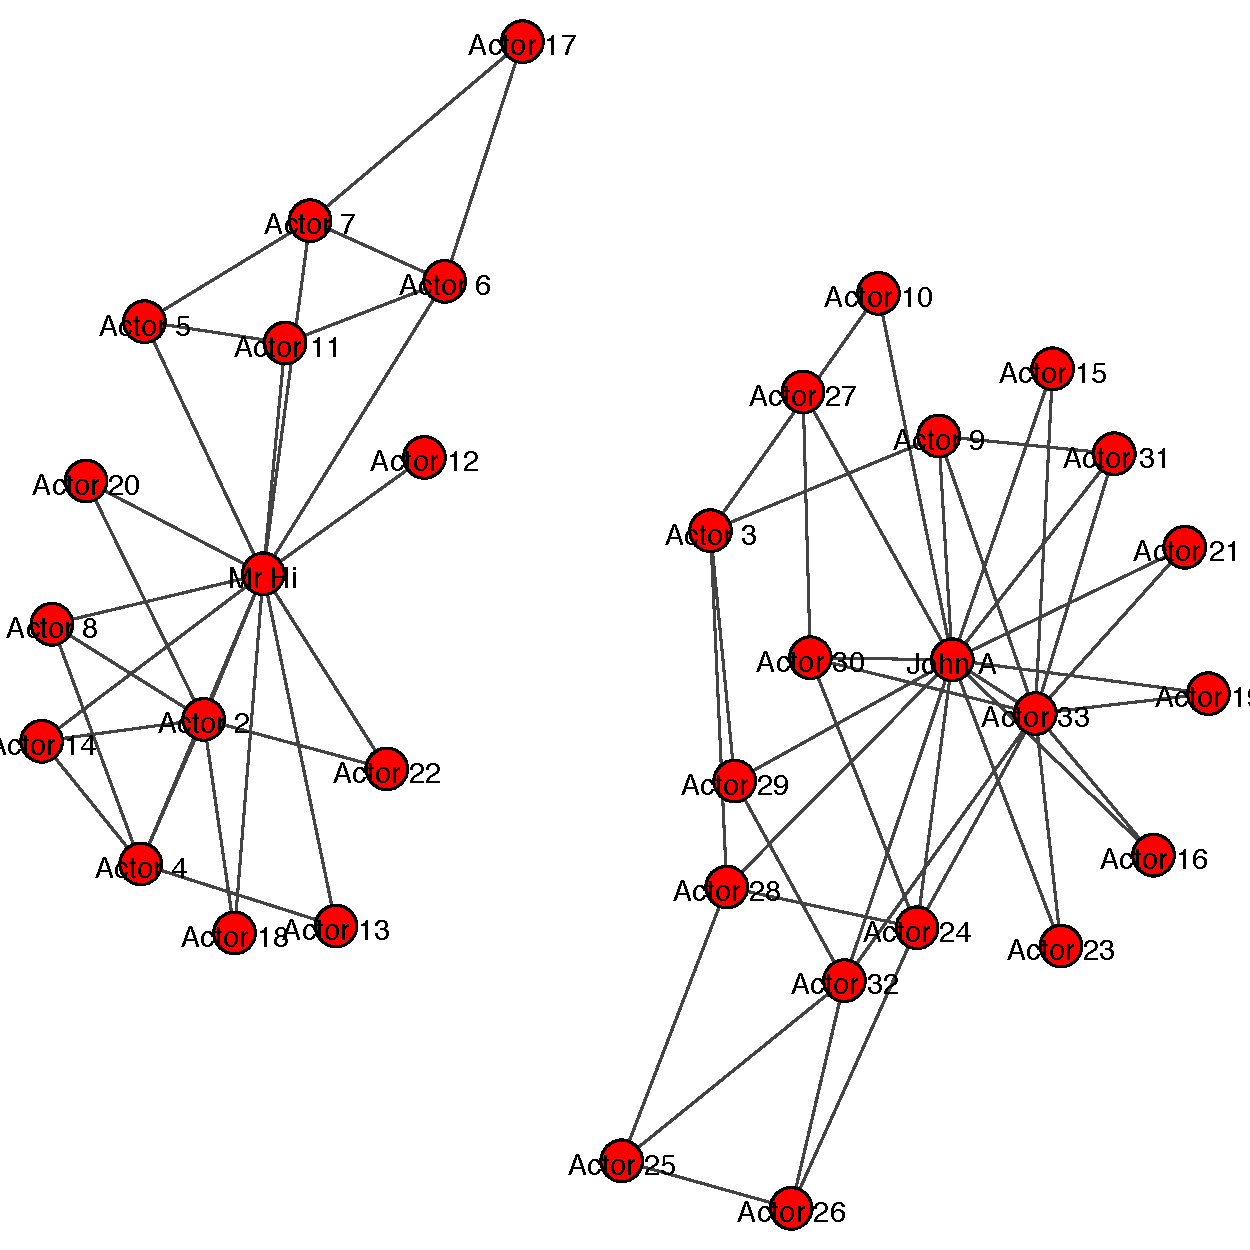
\includegraphics[scale=0.7]{../qn1/finalgraph.pdf}
\centering
\caption{Predicted Seperation using Edge betweenness}
\label{fig:Predicted Seperation using Edge betweenness}
\end{figure}
\newpage
\subsection{Output on console showing removed edges}
\begin{figure}[ht]
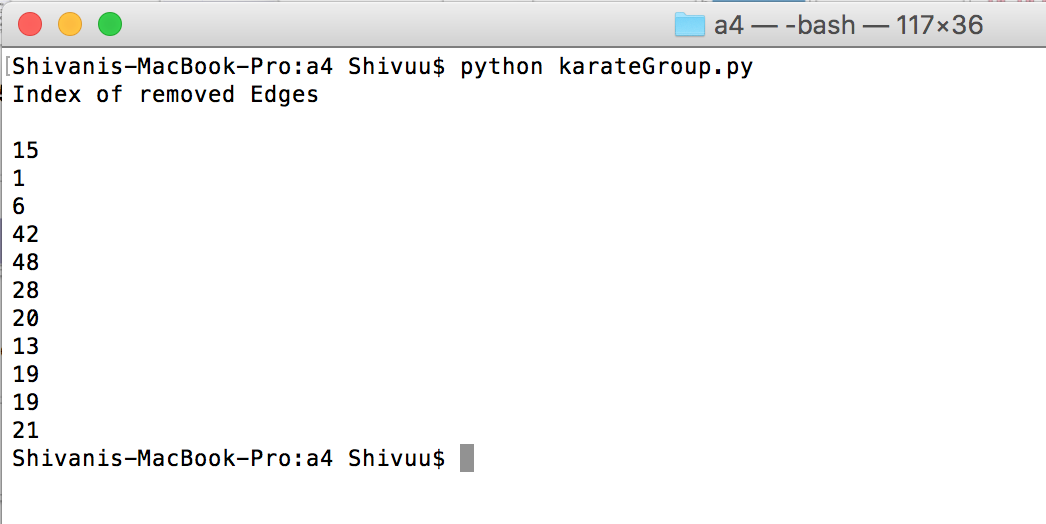
\includegraphics[scale=0.7]{../qn1/screen1.png}
\centering
\caption{Removed edges}
\label{Removed edges}
\end{figure}


\newpage


\newpage




\section{Question 2: }
We know the group split in two different groups.  Suppose the
disagreements in the group were more nuanced -- what would the clubs
look like if they split into groups of 3, 4, and 5?

\subsection{Understanding}
I have decided to follow the same approach I was using earlier to find the two groups. Now, I will have to repeat the loop and delete the edges until I get three, four, five clusters respectively. 

\subsection{Code Listing}
\subsubsection{karateAll.py}
\lstinputlisting[breaklines=True,language=Python]{../qn2/karateAll.py}
\newpage

\subsection{Input}
\subsubsection{karate.GraphML}
\lstinputlisting[breaklines=True]{../qn1/samplegraphML.GraphML}
\newpage

\subsection{Output Files}
\subsubsection{Intial-graph}

 
\begin{figure}[ht]
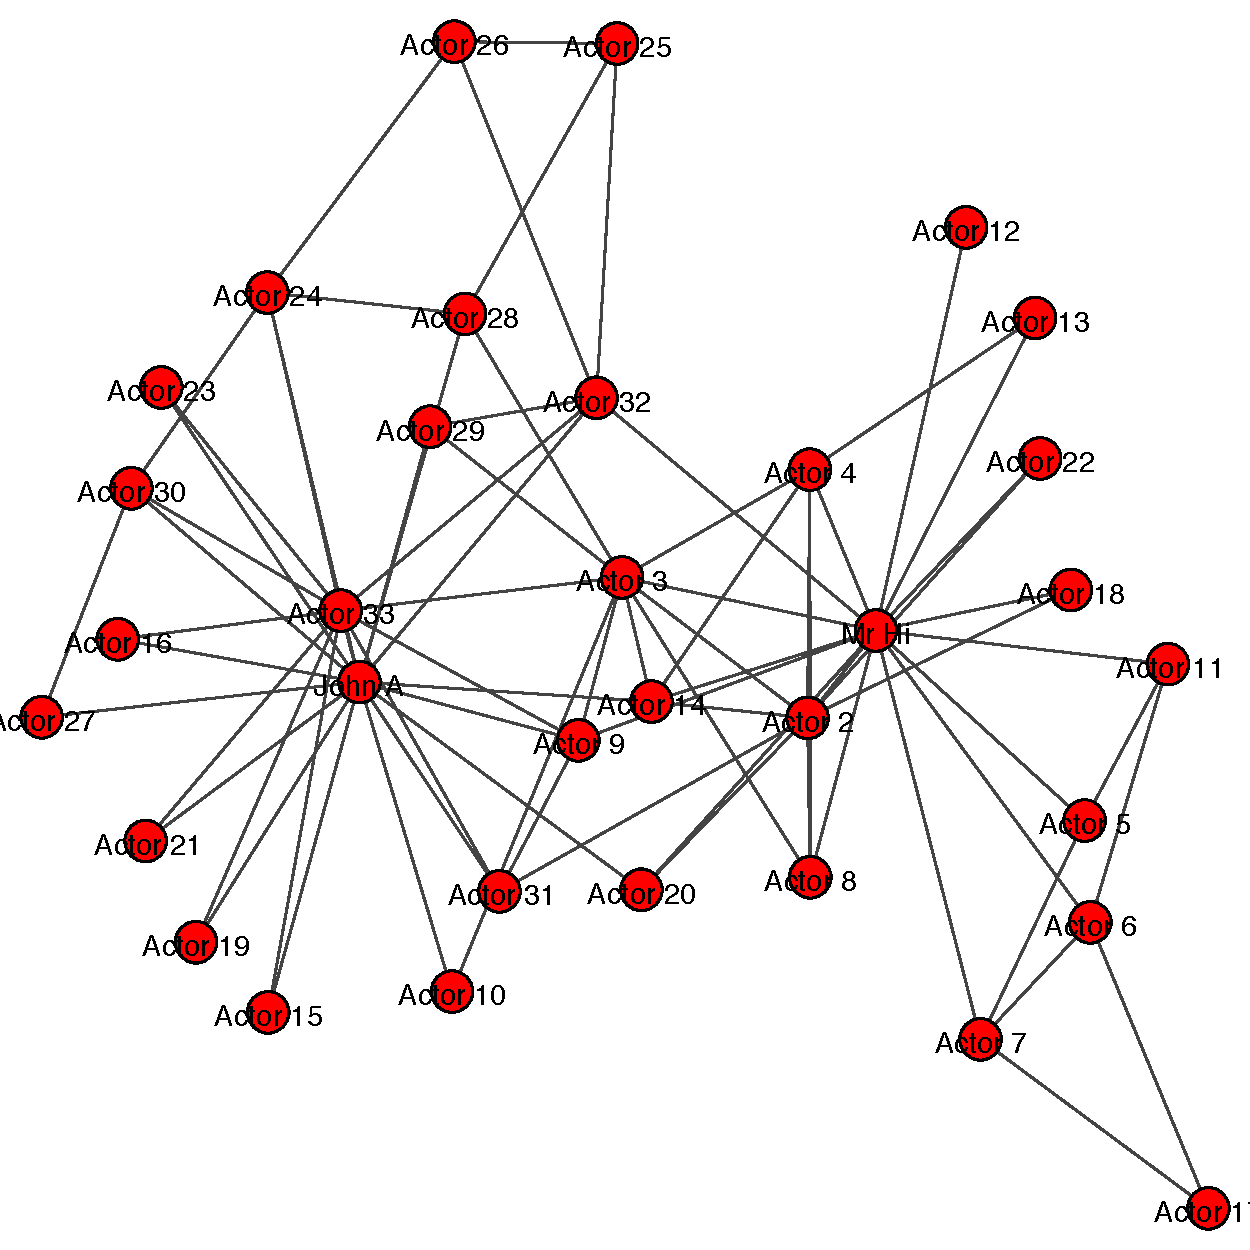
\includegraphics[scale=0.7]{../qn2/graph3.pdf}
\centering
\caption{Initial-graph}
\label{fig:Initial graph}
\end{figure}
\newpage

\subsubsection{Graph after the split}
\begin{figure}[ht]
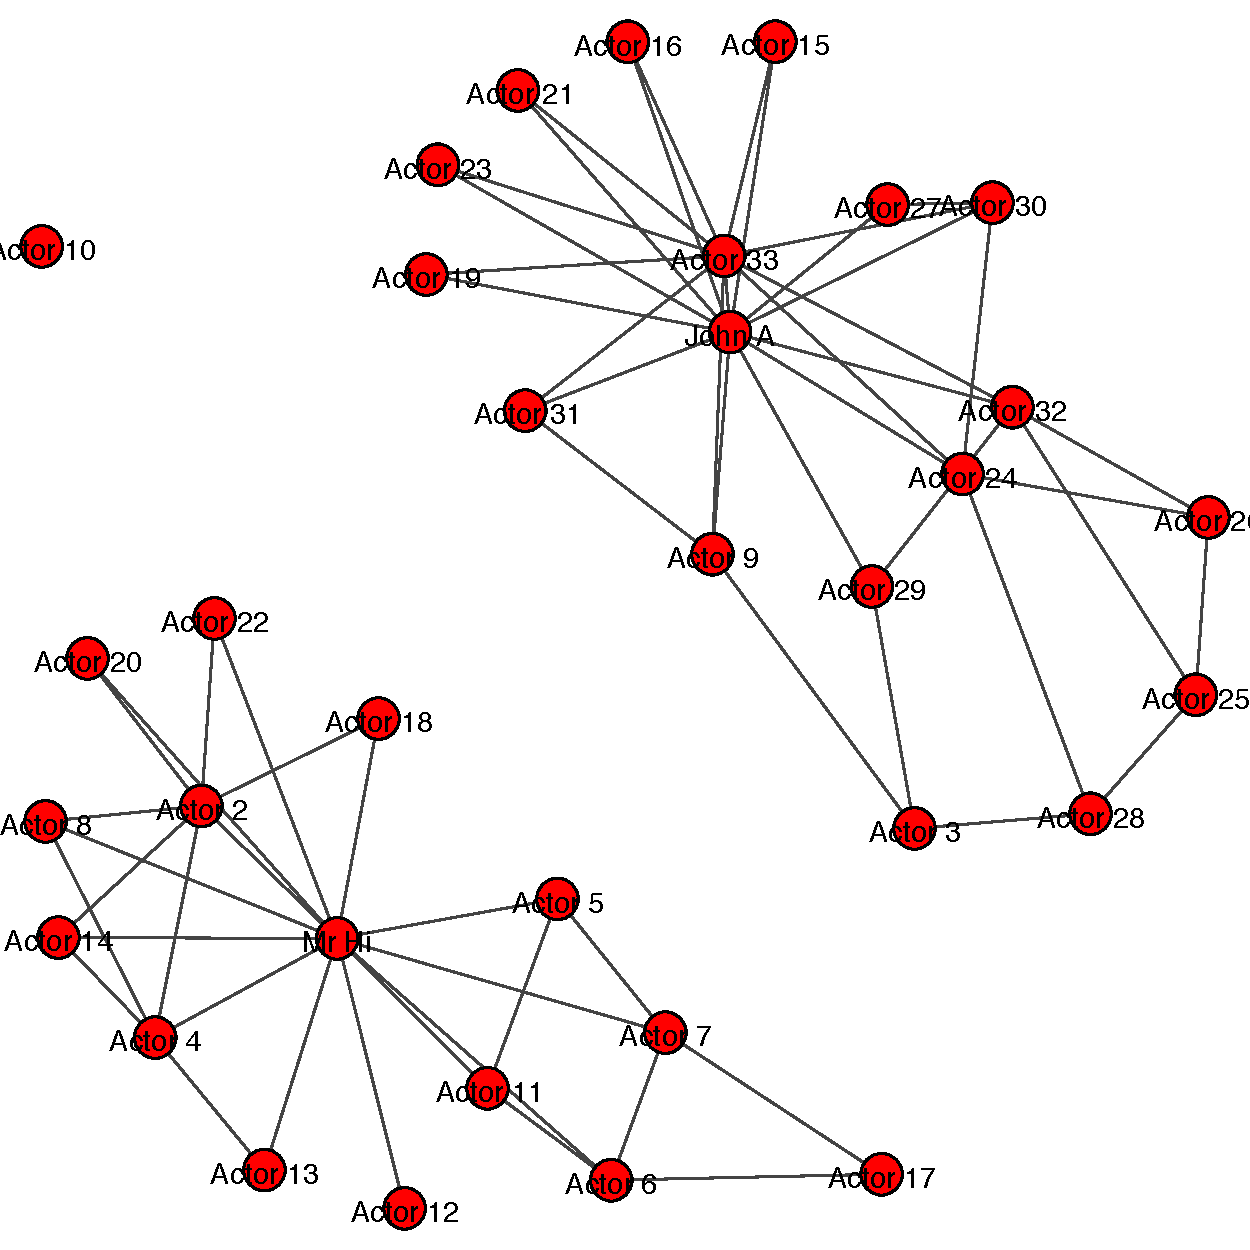
\includegraphics[scale=0.7]{../qn2/finalgraph3.pdf}
\centering
\caption{Initial graph split into 3 groups}
\label{Initial graph split into 3 groups}
\end{figure}
\newpage

\begin{figure}[ht]
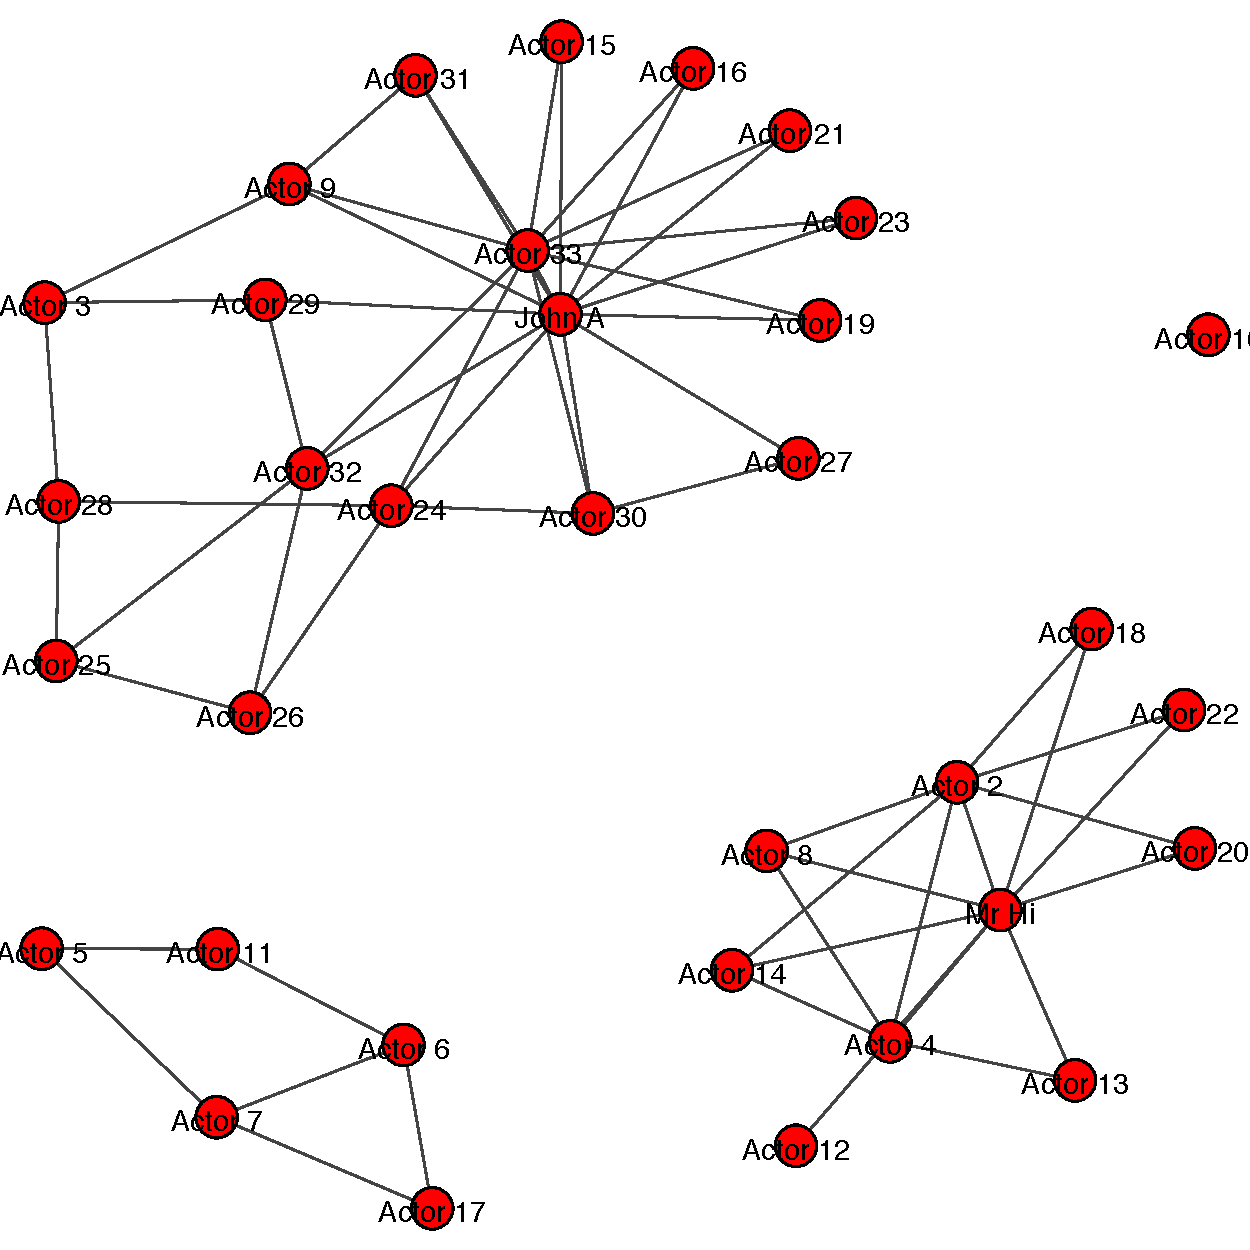
\includegraphics[scale=0.7]{../qn2/finalgraph4.pdf}
\centering
\caption{Initial graph split into 4 groups}
\label{Initial graph split into 4 groups}
\end{figure}
\newpage



\begin{figure}[ht]
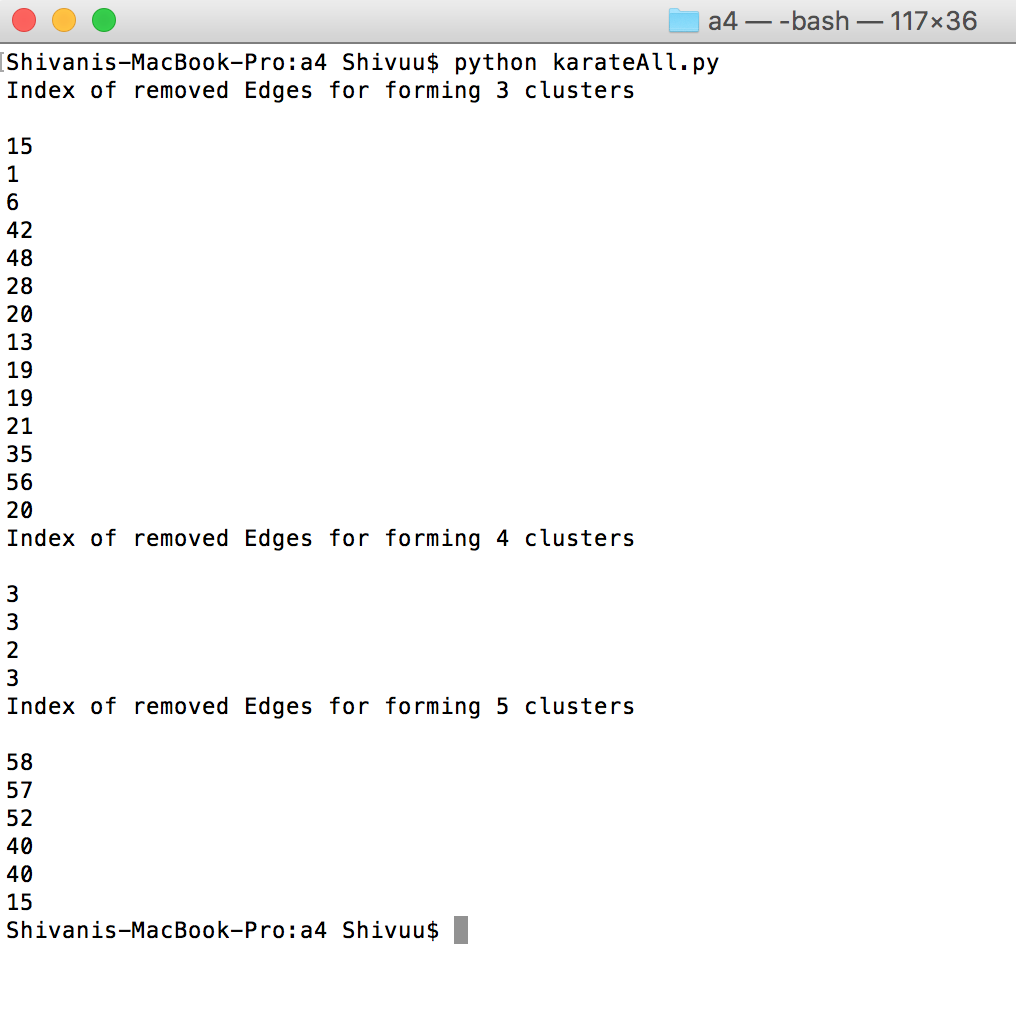
\includegraphics[scale=0.9]{../qn2/screen2.png}
\centering
\caption{Initial graph split into 4 groups}
\label{Initial graph split into 4 groups}
\end{figure}


\addcontentsline{tableofcontents}{section}{References}





\newpage





\bibliographystyle{plain}
\bibliography{references}
\cite{*}
\end{document}